
% plantilla obtenida de: https://www.overleaf.com/19886281jjqffwsxshmm#/73112823/

\documentclass[a4paper, 11pt]{article}
\usepackage{comment} % enables the use of multi-line comments (\ifx \fi) 
\usepackage{lipsum} %This package just generates Lorem Ipsum filler text. 
\usepackage{fullpage} % changes the margin

\usepackage[spanish]{babel}
\usepackage[utf8]{inputenc}
\decimalpoint
\usepackage{graphicx}

\usepackage{amsmath}
\usepackage{amsfonts}
% or
\usepackage{amssymb}
\usepackage{tikz}
\usepackage{array}
\newcolumntype{C}{>{$}l<{$}} % math-mode version of "l" column type
\newcommand{\imageins}[4]{\begin{figure}[!ht]		%Take the hardwork from using images. Let this command do the work for you. Insert images by just using this command \imageins{filename}{width as a ratio of total text width of the page}{caption name}{label name for referring in articles}		
    \centering
    \includegraphics[width=#2\textwidth]{#1}
    %\caption{#3}
    %\label{#4}
    \vspace{0.2em}
\end{figure}}

%%%%%%%%%%%%%%%%%%%%%%%%%%%%%%%%%%%%%%%%%%%%%%%%%%%%%%%%%%%%%%%%%%%%%%%%%%%%%%%%%%
\usepackage{listings}
\usepackage{color}
 
\definecolor{codegreen}{rgb}{0,0.6,0}
\definecolor{codegray}{rgb}{0.5,0.5,0.5}
\definecolor{codepurple}{rgb}{0.58,0,0.82}
\definecolor{backcolour}{rgb}{0.95,0.95,0.92}
 
\lstdefinestyle{mystyle}{
    backgroundcolor=\color{backcolour},   
    commentstyle=\color{codegreen},
    keywordstyle=\color{magenta},
    numberstyle=\tiny\color{codegray},
    stringstyle=\color{codepurple},
    basicstyle=\footnotesize,
    breakatwhitespace=false,         
    breaklines=true,                 
    captionpos=b,                    
    keepspaces=true,                 
    numbers=left,                    
    numbersep=5pt,                  
    showspaces=false,                
    showstringspaces=false,
    showtabs=false,                  
    tabsize=2
}
 
\lstset{style=mystyle}

%%%%%%%%%%%%%%%%%%%%%%%%%%%%%%%%%%%%%%%%%%%%%%%%%%%%%%%%%%%%%%%%%%%%%%%%%%%%%%%%%%

\begin{document}
%Header-Make sure you update this information!!!!
\noindent
\large\textbf{Práctica Lex} \hfill \textbf{Antonio Gámiz Delgado} \\
\normalsize Modelos de Computación \hfill 25/11/2018
%\normalsize ECE 100-003 \hfill Teammates: Student1, Student2 \\
%Prof. Oruklu \hfill Lab Date: XX/XX/XX \\
%TA: Adam Sumner \hfill Due Date: XX/XX/XX

\section*{Objetivo}

En esta práctica he hecho una aplicación con Lex, cuyo principal objetivo es generar, a partir de un archivo de código (\textless file\textgreater.cpp), otro archivo ((\textless file\textgreater.todo) conteniendo los TODOs de ese arvhico, separados por tipos. Además, también añade al final las referencias encontradas.

(1) Los TODO son una forma de anotar tareas o quehaceres en los comentarios de un lenguaje de programación.

\section*{Explicación}

Todos los TODOS empiezan con una cabecera o header, que es de la forma "//TODO:"
\begin{lstlisting}[language=C]
todoHeader {separator}[ ]?"TODO"[ ]?:
\end{lstlisting}

Para detectar si es un comentario o no, usamos la siguiente regex:
\begin{lstlisting}[language=C]
separator (\/\/|#)
\end{lstlisting}
Que detecta comentarios en lenguajes como Java, C, C++, Bash, etc. Además, he usado las siguientes regex auxliares:
\begin{lstlisting}[language=C]
// detecta fechas en el formato dd/mm/yyyy
date {number}{1,2}\/{number}{1,2}\/{number}{4}
any (.+|.?) // cualquier caracter
restoLinea {any}\n // cualquiercaracter + final de linea
\end{lstlisting}


Hay 4 tipos de TODO, que detallaré a continuación:

\begin{itemize}
\item TODO incorrecto, que consiste en una linea en la que sólo aparece el header.
\begin{lstlisting}[language=C]
todoVacio ([ ]?|[ ]+)\n
{todoHeader}[ ]?{todoVacio}
\end{lstlisting}
\item TODO 2, que consiste en el header + una fecha de deadline + palara urgente en algún punto de la cadena.
\begin{lstlisting}[language=C]
todoTipo2  "Deadline":[ ]?{date}{any}"URGENTE"{restoLinea}
{todoHeader}[ ]?{todoTipo2}
\end{lstlisting}
\item TODO 1, que consiste en el header + una fecha de deadline + cualquier cadena.
\begin{lstlisting}[language=C]
todoTipo1  "Deadline":[ ]?{date}{restoLinea}
{todoHeader}[ ]?{todoTipo1}
\end{lstlisting}
\item TODO 0, que consiste en el header + cualquier cadena de caracteres.
\begin{lstlisting}[language=C]
todoTipo0  {restoLinea}
{todoHeader}[ ]?{todoTipo0}
\end{lstlisting}

\end{itemize}

Además de lo anterior, también detecta el uso de referencias de la forma "//See also: url", para detectar urls uso estas regexs:
\begin{lstlisting}[language=C]
letter [a-zA-Z]
number [0-9]

protocol ("http"|"https")"://"
address "www"\..+\.{letter}{1,3}
path \/({letter}|{number})?

url {protocol}{address}{path}?
\end{lstlisting}

Y para las referencias:
\begin{lstlisting}[language=C]
referencia  {separator}?[ ]?"See also:"[ ]?{url}
\end{lstlisting}

En los ficheros adjuntos a esta memoria he añadido un archivo llamado \textit{random.cpp} que contiene código aleatorio junto con TODOs y referencias de prueba, adjunto resultado de la ejecución en el archivo \textit{todos.txt}. El código de la applicación se encuentra en \textit{ToDo.l} y el script \textit{exe.sh} es para compilar y ejecutar más cómodamente la aplicación.

\begin{figure}[h]
\center
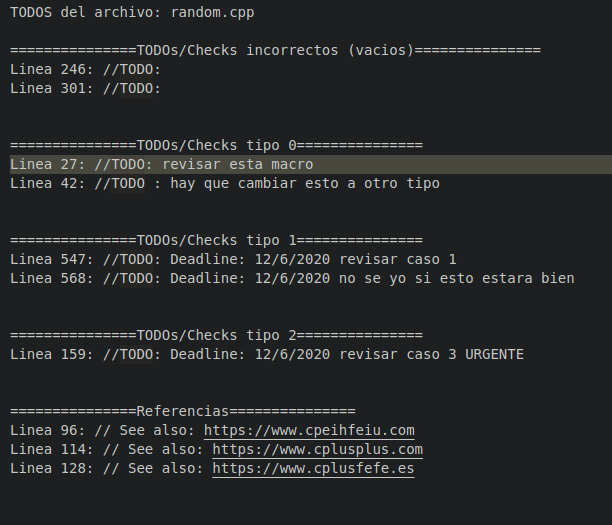
\includegraphics[scale=0.7]{ejemplo}
\caption{Ejemplo de ejecuación con el archivo \textit{random.cpp}}
\end{figure}


\end{document}